\documentclass{cours}

\title{Jeux et Langages Formels}
\author{Matthieu Boyer}
\date{\today}

\markright{Matthieu Boyer}
\pagestyle{myheadings}

\usetikzlibrary{automata, arrows, calc, matrix, positioning}
\definecolor{vulm}{HTML}{7d1dd3}
\definecolor{yulm}{HTML}{ffe500}
\usepackage{caption}

\usepackage{tcolorbox}
\tcbuselibrary{theorems}
\NewTcbTheorem[auto counter, number within=section]{définition}{Définition}%
 {colback=yulm!10, colframe=vulm!45!black, fonttitle=\bfseries}{def}

\NewTcbTheorem[use counter from=définition]{théorème}{Théorème}%
 {colback=yulm!10!white, colframe=vulm!65!black, fonttitle=\bfseries}{thm}

\NewTcbTheorem[use counter from=définition]{propositionfr}{Proposition}%
 {colback=yulm!10!white, colframe=vulm!25!black, fonttitle=\bfseries}{propo}

\NewTcbTheorem[use counter from=définition]{corollaire}{Corollaire}%
 {colback=yulm!10, colframe=vulm!35!black, fonttitle=\bfseries}{cor}

\NewTcbTheorem[use counter from=définition]{lemme}{Lemme}%
 {colback=yulm!10, colframe=vulm!15!black, fonttitle=\bfseries}{lemme}

\NewTcbTheorem[use counter from=définition]{remarque}{Remarque}%
 {colback=yulm!10, colframe=vulm!65!black, fonttitle=\bfseries}{rem}


\begin{document}
\begin{abstract}
    Dans ce rapport, on s'intéresse à des manières de représenter des jeux par la théorie des langages formels, en particulier par les automates et par les automates à pile. On présente alors une nouvelle caractérisation de la régularité d'un langage comme sa reconnaissance par une certaine représentation des jeux. Puis, en modifiant cette représentation, on trouve une caractérisation des langages algébriques par les jeux. Enfin, on s'intéresse à une manière de représenter le \textit{Game Design} par des automates en introduisant un délai sur les transitions, et on regarde quelques exemples d'applications.
\end{abstract}

\section*{Introduction}
Dans la suite on ne s'intéresse qu'à des jeux à plusieurs joueurs i.e. plus de deux.\\
Un jeu à plusieurs joueurs est, de manière informelle, une abstraction d'un jeu ressemblant par exemple à la belote : chaque joueur, à son tour, va choisir, parmi un éventail de coups possibles, celui qu'il souhaite effectuer, modifiant alors l'état du jeu. En reprenant l'exemple de la belote, un coup est une carte de la main du joueur, qui ne sait pas exactement quelles cartes ont ses adversaires, et qui ne peut la jouer que sous certaines conditions, à résoudre dans l'ordre :
\begin{enumerate}
    \item Soit il est le premier à jouer
    \item Soit la carte est de la \textit{bonne} couleur
    \item Soit la carte est un atout plus grand que le dernier joué
    \item Soit la carte est une coupe (atout lorsqu'une autre couleur est jouée)
    \item Soit il ne peut rien jouer d'autre remplissant les conditions précédentes
\end{enumerate}
Il paraît alors raisonnable qu'en limitant les transitions possibles de l'état de jeu selon l'état et selon les règles du jeu, on puisse modéliser un jeu par un automate. Toutefois, le manque d'informations d'un joueur sur les mains de ses adversaires, semble aussi limiter la description directe du jeu avec un caractère non-déterministe. \\
On s'intéresse donc ici à des manières de décrire les jeux par les automates et les grammaires formelles.

\newpage
\section{Jeux et Automates}
\subsection{Première définition de Jeu}
On introduit d'abord une première définition de jeu suivant \cite{game-rep-automata}:
\begin{définition}{Première définition de Jeu}{}
    Un jeu est un triplet $\left(P, A_{i}, \succeq_{i}\right)$ où $P$ est un ensemble de joueurs, $A_{i}$ est un ensemble d'actions pour le joueur $i \in P$ et $\succeq_{i}$ est une relation de préférence pour le joueur $i$.
\end{définition}

Pour le \textsc{Dilemme du Prisonnier}, on a par exemple : $P = \left\{1, 2\right\}$, $\forall i, A_{i} = \left\{A, N\right\}$ et $\succeq_{i}$ peut se lire sur l'arbre de jeu \ref{fig:gametree:full_info_pridi} de manière numérique.
\begin{figure}
    \centering
    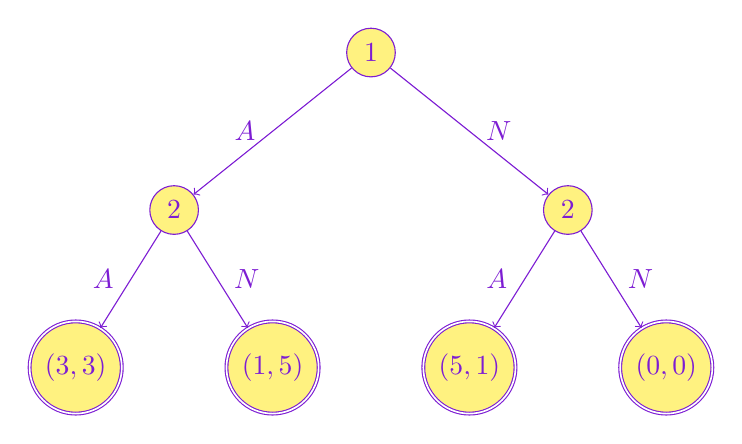
\begin{tikzpicture}[level distance=2cm,
            level 1/.style={sibling distance=5cm},
            level 2/.style={sibling distance=2.5cm}]
        \tikzstyle{every node}=[circle,draw = vulm, fill = yulm!50, text = vulm]
        \node {1}
        child[vulm] {node {2}
                child[vulm] {node[double] {$(3, 3)$} edge from parent[->] node[left, draw = none, fill = none] {$A$}}
                child[vulm] {node[double] {$(1, 5)$} edge from parent[->] node[right, draw = none, fill = none] {$N$}}
                edge from parent[->] node[left, draw = none, fill = none] {$A$}
            }
        child[vulm] {node {2}
                child[vulm] {node[double] {$(5, 1)$} edge from parent[->] node[left, draw = none, fill = none] {$A$}}
                child[vulm] {node[double] {$(0, 0)$} edge from parent[->] node[right, draw = none, fill = none] {$N$}}
                edge from parent[->] node[right, draw = none, fill = none ] {$N$}
            };
    \end{tikzpicture}
    \caption{Représentation Extensive du Jeu du \textsc{Dilemme du Prisonnier} à information totale.}
    \label{fig:gametree:full_info_pridi}
\end{figure}

Ici, chaque noeud interne de l'arbre correspond à un joueur, chaque arête à un coup qu'il peut jouer, c'est-à-dire dans notre cas, choisir d'avouer ($A$) son crime, ou bien de le nier ($N$) et les feuilles de l'arbre représentent les résultats, cf. Table \ref{table:full_info_pridi}.\\
\begin{table}[ht]
    \centering
    \caption{Résultats du \textsc{Dilemme du Prisonnier}}
    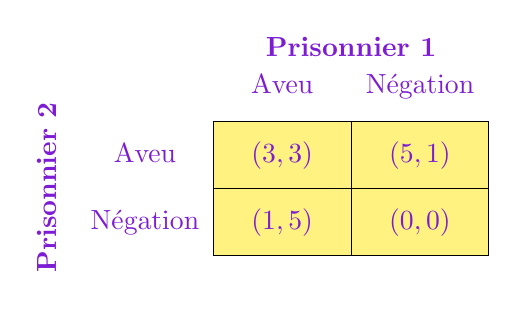
\begin{tikzpicture}[element/.style={minimum width=1.75cm,minimum height=0.85cm}]
        \matrix (m) [matrix of nodes,nodes={element},column sep=-\pgflinewidth, row sep=-\pgflinewidth, text = vulm]{
        & Aveu & Négation \\
        Aveu & |[draw, fill = yulm!50]|$(3, 3)$ & |[draw, fill = yulm!50]|$(5, 1)$ \\
        Négation & |[draw, fill = yulm!50]|$(1, 5)$ & |[draw, fill = yulm!50]|$(0, 0)$ \\    };

        \node[above=0.25cm, text = vulm] at ($(m-1-2)!0.5!(m-1-3)$){\textbf{Prisonnier 1}};
        \node[rotate=90, text = vulm] at ($(m-2-1)!0.5!(m-3-1)+(-1.25,0)$){\textbf{Prisonnier 2}};
    \end{tikzpicture}
    \label{table:full_info_pridi}
\end{table}
\begin{définition}{Description Extensive}{}
    On appelle la description d'un jeu à information totale sous forme d'arbre (cf. figure \ref{fig:gametree:full_info_pridi} ) précédente la description extensive de ce jeu.
\end{définition}

Toutefois, d'autre descriptions peuvent être préférables, notamment lorsque l'un des joueurs n'a pas d'information sur les coups des autres joueurs, comme c'est le cas dans certaines variantes du \textsc{Dilemme du Prisonnier}. En effet, on considérait ici que le prisonnier numéro\footnote{NDA : \textit{I am not a number ! I am a free man !}} $2$ est informé du choix du prisonnier numéro $1$, ce qui n'est pas un très bon choix de la part des geôliers.
\begin{définition}{Information d'un Jeu}{}
    On parle de jeu à information imparfaite (par opposition aux jeux à information totale), lorsque le joueur actuel n'a pas d'informations sur les coups des joueurs précédents. On représente ceci en rajoutant sur l'arbre de jeu l'information possédée par un joueur lors de son coup en entourant l'ensemble des positions possibles.
\end{définition}

Dans le cas du \textsc{Dilemme du Prisonnier}, on modifie l'arbre \ref{fig:gametree:full_info_pridi} comme suit :
\begin{figure}
    \centering
    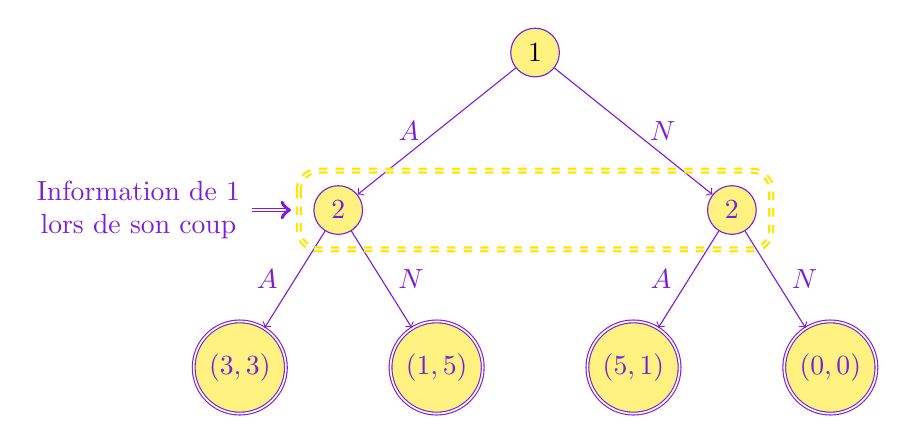
\begin{tikzpicture}[level distance=2cm,
            level 1/.style={sibling distance=5cm},
            level 2/.style={sibling distance=2.5cm}]
        \tikzstyle{every node}=[circle,draw = vulm, fill = yulm!50]
        \node(0) {1}
        child[vulm] {node {2}
                child[vulm] {node[double] {$(3, 3)$} edge from parent[->] node[left, draw = none, fill = none] {$A$}}
                child[vulm] {node[double] {$(1, 5)$} edge from parent[->] node[right, draw = none, fill = none] {$N$}}
                edge from parent[->] node[left, draw = none, fill = none] {$A$}
            }
        child[vulm] {node {2}
                child[vulm] {node[double] {$(5, 1)$} edge from parent[->] node[left, draw = none, fill = none] {$A$}}
                child[vulm] {node[double] {$(0, 0)$} edge from parent[->] node[right, draw = none, fill = none] {$N$}}
                edge from parent[->] node[right, draw = none, fill = none] {$N$}
            };
        \draw[dashed,rounded corners=7, double, yulm, thick = 2pt]($(0-1)+(-.5,.5)$)rectangle($(0-2)+(.5,-.5)$);
        \tikzstyle{every node} = []
        \node at ($(0-1) + (-1,.)$)[label ={[align = center, vulm]left : Information de $1$\\ lors de son coup}]{};
        \draw[->, double, distance = 5pt, vulm]($(0-1) + (-1.1,.)$)--($(0-1)+(-.6,.)$);
    \end{tikzpicture}
    \caption{Représentation Extensive du Jeu du \textsc{Dilemme du Prisonnier} à information imparfaite.}
    \label{fig:gametree:impinfopridi}
\end{figure}
\begin{définition}{Partie sur un Jeu}{}
    Une partie sur un jeu est une suite d'états de ce jeu, ou, de manière équivalente, une suite de coups $s_{0}s_{1}\ldots s_{k}$ tels que :
    \begin{itemize}
        \item $\forall i, s_{2i} \in A_{0}$ et $s_{2i + 1} \in A_{1}$.
        \item $\not{\exists} s_{k + 1} \in A_{i}$ où $i = 1$ si $k \equiv 0 \mod 2$ et $i = 0$ sinon.
    \end{itemize}
\end{définition}

\subsection{Les Automates vus comme des Jeux}
\begin{définition}{Jeu d'un Automate}{}
    Si $A = \left(Q, \Sigma, \delta, q_{0}, F\right)$ est un automate, on se donne $G_{A}$ un jeu sous représentation extensive à deux joueurs \textsc{Tatiana} et \textsc{Pierre}. Dans ce jeu, \textsc{Tatiana} joue des états de $Q$ et \textsc{Pierre} joue des lettres de $\Sigma$.
\end{définition}
On joue comme suit :
\begin{itemize}
    \item \textsc{Tatiana} joue $q_{0}$ l'état initial.
    \item \textsc{Pierre} doit jouer une lettre $s \in \Sigma$
    \item La partie se termine lorsque \textsc{Tatiana} joue un état de $F$ et que \textsc{Pierre} n'a plus de coup valable.
\end{itemize}

\begin{définition}{Règles du Jeu}{}
    Les règles du jeu pour chaque joueur sont les suivantes : si \textsc{Tatiana} joue $q \in \Sigma$ alors \textsc{Pierre} doit jouer $s$ tel que $\delta(q, s) \neq \emptyset$ sinon il perd.
\end{définition}

On peut par ailleurs faire un lien entre le caractère déterministe de l'automate et l'information donnée au joueur \textsc{Pierre}, ce qui correspond intuitivement au fait qu'on puisse aller d'un état à plusieurs.
\begin{itemize}
    \item Si $A$ est déterministe, $G_{A}$ est équivalent à un jeu à information parfaite, puisqu'en effet, après le coup de l'adversaire, on peut être certain de l'état du jeu.
    \item A l'inverse, si $A$ n'est pas déterministe, on peut d'une meilleure manière définir des ensembles d'informations pour chacun des joueurs récursivement : On a en effet : $\delta(q, s) = B \subseteq Q$ et on a alors un ensemble d'informations autour du prochain coup de \textsc{Pierre} lorsque \textsc{Tatiana} joue $q' \in B$. En effet, \textsc{Pierre} doit alors jouer $s' \in \Sigma$ tel que $\delta(q, s')$ est défini et $q \in B$.
\end{itemize}
Dans la suite, on se place d'abord dans le cas déterministe.\\
Pour l'automate de la figure \ref{fig:dfa1}, 
\begin{figure}
    \centering
    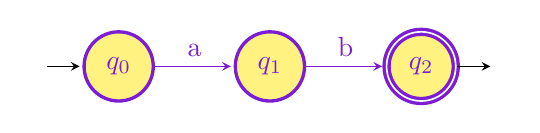
\begin{tikzpicture}[shorten >=1pt,node distance=1cm,>={stealth}, initial text = ,
        every state/.style={draw=vulm,very thick,fill=yulm!50, text = vulm}, accepting/.style={accepting by arrow, double}]
        \node[state, initial] (q_0) {$q_{0}$};
        \node[state] (q_1) [right=of q_0] {$q_{1}$};
        \node[state, accepting] (q_2) [right = of q_1] {$q_{2}$};
        \path[->, vulm] (q_0) edge node [above] {a} (q_1)
        (q_1) edge node [above] {b} (q_2);
    \end{tikzpicture}
    \caption{Un Automate Déterministe}
    \label{fig:dfa1}
\end{figure}
on obtient la représentation extensive de la figure \ref{fig:gametree:dfa1}, en utilisant $\lambda$ comme symbole pour signifier que \textsc{Pierre} n'a plus de lettres jouables :
\begin{figure}
    \centering
    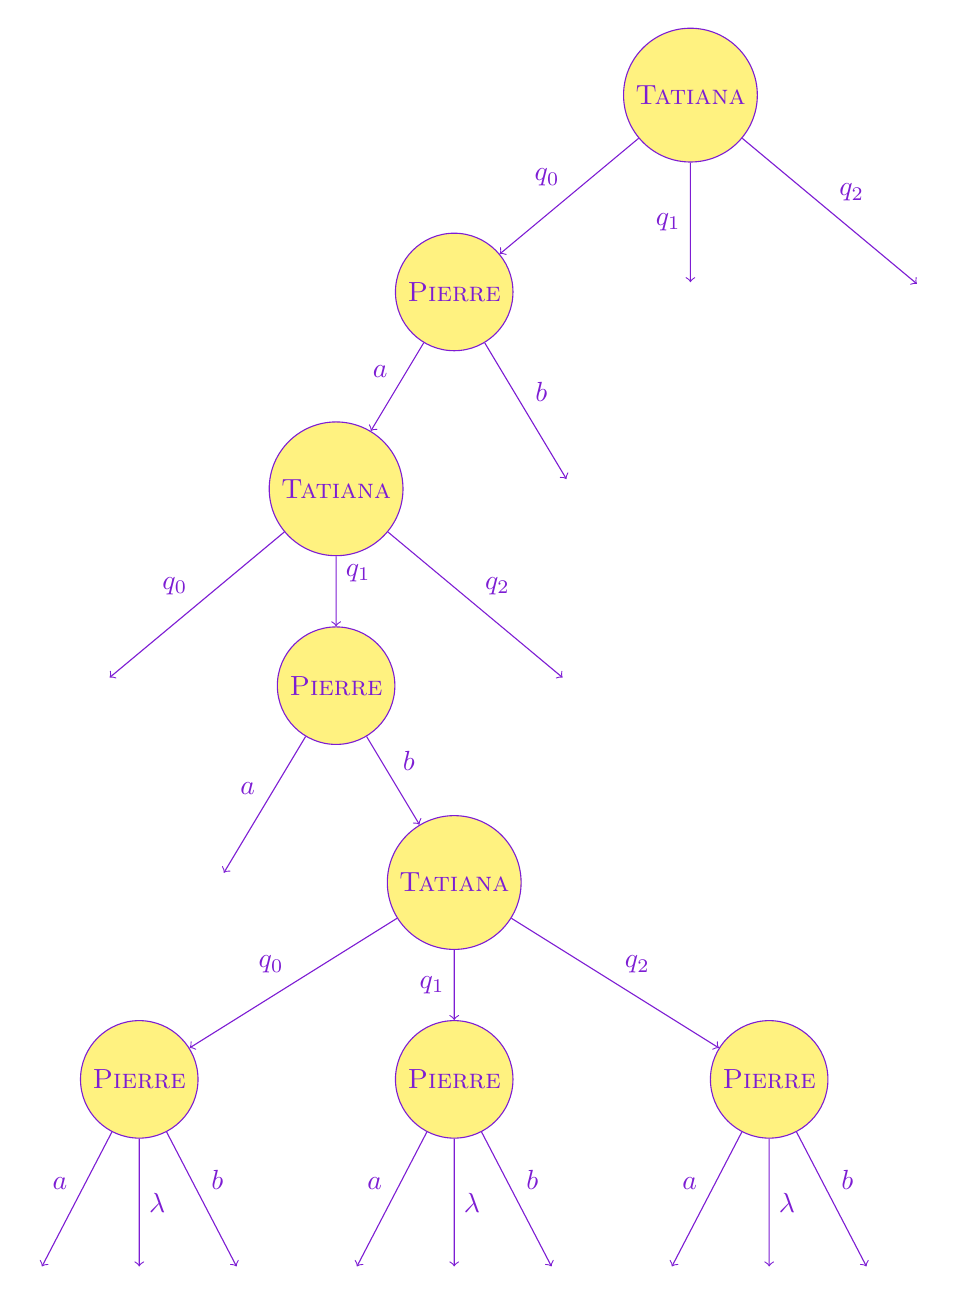
\begin{tikzpicture}[level distance=2.5cm,
            level 1/.style={sibling distance=3cm},
            level 2/.style={sibling distance=3cm},
            level 3/.style={sibling distance=3cm},
            level 4/.style={sibling distance=3cm},
            level 5/.style={sibling distance=4cm},
            level 6/.style={sibling distance=1.3cm}]
        \tikzstyle{every node}=[draw = none, fill = none]
        \node[circle, draw = vulm, fill=yulm!50, text = vulm] {\textsc{Tatiana}}
        child[vulm] {node[circle, draw = vulm, fill=yulm!50] {\textsc{Pierre}}
        child[vulm] {node[circle, draw = vulm, fill=yulm!50] {\textsc{Tatiana}}
        child[vulm] {node {} edge from parent[->] node[above left] {$q_{0}$}}
        child[vulm] {node[circle, draw = vulm, fill=yulm!50] {\textsc{Pierre}}
        child[vulm] {node {} edge from parent[->] node[above left] {$a$}}
        child[vulm] {node[circle, draw = vulm, fill=yulm!50] {\textsc{Tatiana}}
        child[vulm] {node[circle, draw = vulm, fill=yulm!50] {\textsc{Pierre}}
        child[vulm] {node {} edge from parent[->]node[above left]{$a$}}
        child[vulm] {node {} edge from parent[->]node[right]{$\lambda$}}
        child[vulm] {node {} edge from parent[->]node[above right]{$b$}}
        edge from parent[->] node[above left] {$q_{0}$}}
        child[vulm] {node[circle, draw = vulm, fill=yulm!50] {\textsc{Pierre}}
        child[vulm] {node {} edge from parent[->]node[above left]{$a$}}
        child[vulm] {node {} edge from parent[->]node[right]{$\lambda$}}
        child[vulm] {node {} edge from parent[->]node[above right]{$b$}}
        edge from parent[->] node[left] {$q_{1}$}}
        child[vulm] {node[circle, draw = vulm, fill=yulm!50] {\textsc{Pierre}}
        child[vulm] {node {} edge from parent[->]node[above left]{$a$}}
        child[vulm] {node {} edge from parent[->]node[right]{$\lambda$}}
        child[vulm] {node {} edge from parent[->]node[above right]{$b$}}
        edge from parent[->] node[above right] {$q_{2}$}}
        edge from parent[->] node[above right] {$b$}}
        edge from parent[->] node[above right] {$q_{1}$}
        }
        child[vulm] {node {} edge from parent[->] node[above right] {$q_{2}$}}
        edge from parent[->] node[above left] {$a$}
        }
        child[vulm] {node {} edge from parent [->] node[above right] {$b$}}
        edge from parent[->] node[above left] {$q_{0}$}}
        child[vulm] {node {} edge from parent [->] node[left] {$q_{1}$}}
        child[vulm] {node {} edge from parent [->] node[above right] {$q_{2}$}};
    \end{tikzpicture}
    \caption{Représentation Extensive du Jeu à Information Parfaite de l'automate figure \ref{fig:dfa1}}
    \label{fig:gametree:dfa1}
\end{figure}

\subsection{Langage et Stratégies Gagnantes}
On se place ici dans le cas déterministe :\\
On définit formellement la notion de stratégie d'un joueur sur un tel jeu. La stratégie d'un joueur assigne une action choisie par le joueur pour chaque historique des coups dans lequel c'est à son tour de jouer. L'historique d'un joueur est l'ensemble des actions qu'il peut choisir de faire durant la partie. Pour \textsc{Tatiana}, c'est l'ensemble des combinaisons d'états qu'il peut utiliser pour affronter \textsc{Pierre} et pour \textsc{Pierre}, c'est n'importe quel mot $w \in \Sigma^{\star}$ :
\begin{définition}{Stratégie}{}
    Une stratégie pour \textsc{Pierre} définie par $w \in \Sigma^{\star}$ est telle que \textsc{Pierre} joue les lettres de $w$ indépendamment de ce que \textsc{Tatiana} joue.
\end{définition}
On a besoin de se restreindre à des mots de longueur finie $n$ pour les stratégies pour pouvoir vérifier l'équivalence entre l'acception par $A$ et le fait d'être une stratégie gagnante.
\begin{définition}{Stratégie Gagnante}{}
    Une stratégie gagnante pour \textsc{Pierre} est une stratégie $w$ de longueur $n$ où \textsc{Tatiana} n'a pas de coup valide (i.e. la partie est arrivée à son terme) et où son dernier coup est un état final de $A$.
    On définit alors : $S\left(G_{A}\right)^{n}$ l'ensemble des parties gagnantes pour \textsc{Pierre} sur $G_{A}$ où \textsc{Pierre} joue selon un mot de longueur $n$, et $L(A)^{n}$ l'ensemble des mots de longueur $n$ reconnus par $A$.
\end{définition}

Ainsi, on doit montrer qu'étant donnée une stratégie gagnante $s \in S\left(G_{A}\right)^{n}$, il existe un mot $w$ de longueur $n$ accepté par $A$.
On a alors :
\begin{théorème}{Reconnaissance des Stratégies}{}
    $S(G_{A})^{n} = L(A)^{n}$
\end{théorème}
\begin{proof}
    En effet, il est clair qu'on peut trouver une équivalence entre le calcul d'un mot $w$ sur $A$ et le déroulement d'une partie où \textsc{Pierre} joue selon $w$. Ceci se lit sur l'arbre de jeu.
\end{proof}

\subsection{Non-Déterminisme}
On considère désormais le cas des automates finis non-déterministes (NFA). S'ils n'apportent pas d'expressivité, ils permettent tout de même un point de vue intéressant.
\begin{définition}{Jeu d'un NFA}{}
    Etant donné un automate non-déterministe $A$, on définit :
    \begin{itemize}
        \item $P$ un ensemble de deux joueurs où \textsc{Tatiana} joue des états et \textsc{Pierre} des lettres.
        \item Un ensemble $I$ d'ensembles d'informations $B$, où on définit $\delta\left(q, s\right) = B$ lorsqu'il y a du non-déterminisme dans la transition.
        \item Des relations de préférence $\succeq_{i}$ entre deux transitions $\delta_{1}, \delta_{2}$ où $\delta_{1} \succeq \delta_{2}$ si et seulement si $d\left(\delta_{1}\right) \leq d(\delta_{2})$ où $d(\tau)$ renvoie la distance dans l'automate vu comme un graphe orienté entre l'état de fin de $\tau$ et son état de début.
    \end{itemize}
\end{définition}

Pour l'automate de la figure \ref{fig:nfa1}
\begin{figure}
    \centering
    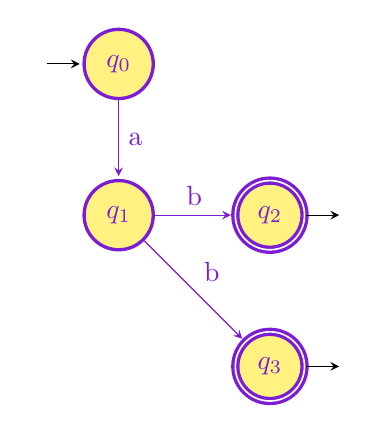
\begin{tikzpicture}[shorten >=1pt,node distance=1cm,>={stealth}, initial text = ,
        every state/.style={draw=vulm,very thick,fill=yulm!50, text = vulm}, accepting/.style={accepting by arrow, double}]
        \node[state, initial] (q_0) {$q_{0}$};
        \node[state] (q_1) [below=of q_0] {$q_{1}$};
        \node[state, accepting] (q_2) [right=of q_1] {$q_{2}$};
        \node[state, accepting] (q_3) [below=of q_2] {$q_{3}$};
        \path[->, vulm] (q_0) edge node [right] {a} (q_1)
        (q_1) edge node [above] {b} (q_2)
        (q_1) edge node [above right] {b} (q_3);
    \end{tikzpicture}
    \caption{Un Automate Non-Déterministe}
    \label{fig:nfa1}
\end{figure}
on obtient l'arbre de la figure \ref{fig:gametree:nfa1}.
\begin{figure}
    \centering
    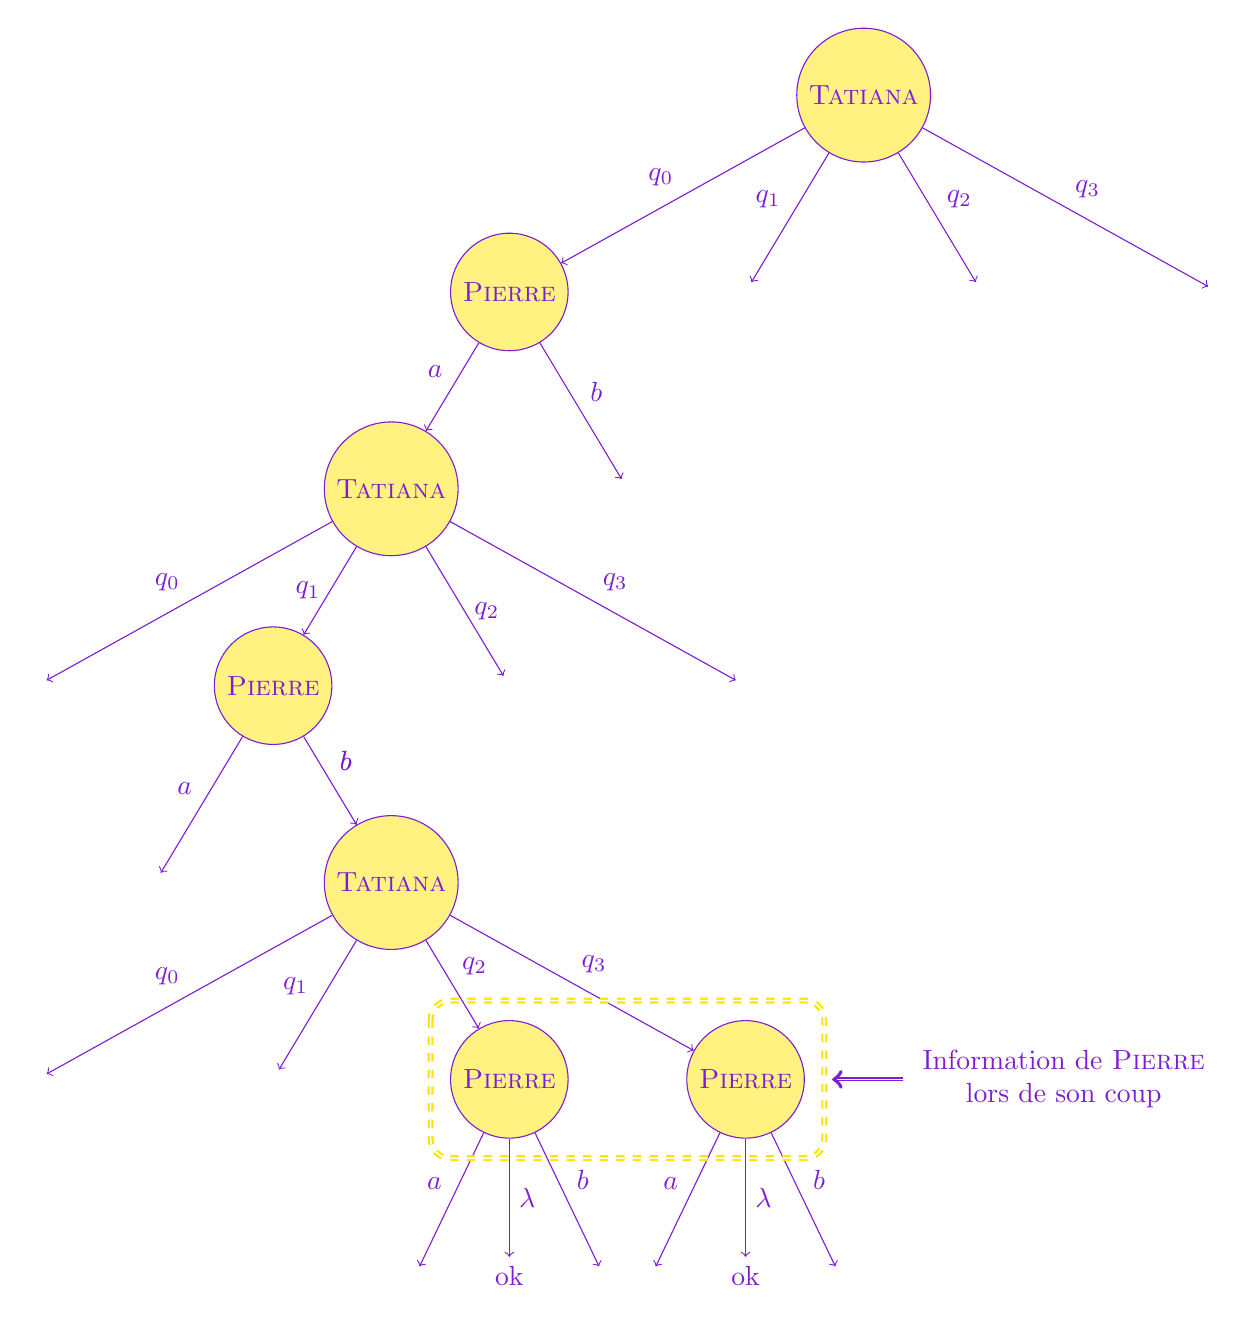
\begin{tikzpicture}[level distance=2.5cm,
            level 1/.style={sibling distance=3cm},
            level 2/.style={sibling distance=3cm},
            level 3/.style={sibling distance=3cm},
            level 4/.style={sibling distance=3cm},
            level 5/.style={sibling distance=3cm},
            level 6/.style={sibling distance=1.2cm}
        ]
        \tikzstyle{every node}=[draw = none, fill = none]
        \node[circle, draw = vulm, fill=yulm!50, text = vulm] (0) {\textsc{Tatiana}}
            child[vulm] {node[circle, draw = vulm, fill=yulm!50] {\textsc{Pierre}}
                child[vulm] {node[circle, draw = vulm, fill=yulm!50] {\textsc{Tatiana}}
                    child[vulm] {node {} edge from parent[->] node[above left] {$q_{0}$}}
                    child[vulm] {node[circle, draw = vulm, fill=yulm!50] {\textsc{Pierre}}
                        child[vulm] {node {} edge from parent[->] node[above left] {$a$}}
                        child[vulm] {node[circle, draw = vulm, fill=yulm!50] {\textsc{Tatiana}}
                            child[vulm] {node {} edge from parent[->] node[above left] {$q_{0}$}}
                            child[vulm] {node {} edge from parent[->] node[above left] {$q_{1}$}}
                            child[vulm] {node[circle, draw = vulm, fill=yulm!50](l) {\textsc{Pierre}}
                                child[vulm] {node {} edge from parent[->]node[above left]{$a$}}
                                child[vulm] {node {ok} edge from parent[->]node[right]{$\lambda$}}
                                child[vulm] {node {} edge from parent[->]node[above right]{$b$}}
                                edge from parent[->] node[above right] {$q_{2}$}}
                            child[vulm] {node[circle, draw = vulm, fill=yulm!50](r) {\textsc{Pierre}}
                                child[vulm] {node {} edge from parent[->]node[above left]{$a$}}
                                child[vulm] {node {ok} edge from parent[->]node[right]{$\lambda$}}
                                child[vulm] {node {} edge from parent[->]node[above right]{$b$}}
                                edge from parent[->] node[above right] {$q_{3}$}}
                            edge from parent[->] node[above right] {$b$}
                            edge from parent[->] node[above right] {$b$}}
                        edge from parent[->] node[left] {$q_{1}$}
                    }
                    child[vulm] {node {} edge from parent[->] node[right] {$q_{2}$}}
                    child[vulm] {node {} edge from parent[->] node[above right] {$q_{3}$}}
                    edge from parent[->] node[above left] {$a$}
                }
                child[vulm] {node {} edge from parent [->] node[above right] {$b$}}
                edge from parent[->] node[above left] {$q_{0}$}}
            child[vulm] {node {} edge from parent [->] node[above left] {$q_{1}$}}
            child[vulm] {node {} edge from parent [->] node[above right] {$q_{2}$}}
            child[vulm] {node {} edge from parent [->] node[above right] {$q_{3}$}};
        
        \draw[dashed, rounded corners=7, thick = 2pt, double, draw = yulm]($(l)+(-1,1)$)rectangle($(r)+(1,-1)$);
        \node at ($(r) + (2,.)$)[label ={[align = center, vulm]right : Information de \textsc{Pierre}\\ lors de son coup}]{};
        \draw[->, double, distance = 5pt, vulm]($(r) + (2.,.)$)--($(r)+(1.1,.)$);
    \end{tikzpicture}
    \caption{Représentation Extensive du Jeu à Information Imparfaite de l'Automate figure \ref{fig:nfa1}}
    \label{fig:gametree:nfa1}
\end{figure}
On vérifie bien sur la figure \ref{fig:gametree:nfa1} qu'il n'y a pas besoin d'indiquer les ensembles d'informations sur les autres étapes du jeu.\\
On remarque par ailleurs, qu'en reprenant les définitions précédentes, on obtient bien le même théorème d'équivalence entre les stratégies gagnantes et les mots acceptés. Ceci se comprend quitte à déterminiser l'automate. On obtient donc en particulier le théorème suivant : 
\begin{théorème}{Information et Reconnaissance}{}
    Tout jeu à information imparfaite est équivalent, au sens de la reconnaissance des langages, à un jeu à information totale. 
\end{théorème}

\newpage
\section{Jeux et Grammaires}
On s'intéresse désormais à une nouvelle définition de jeu, les jeux hors-contexte, qu'on va écrire avec des automates à pile (et donc des grammaires), et on verra ensuite une application à deux jeux de cartes particuliers : le \textsc{Uno} et le \textsc{Texas Hold'Em Poker}. 
\subsection{Jeux Hors-Contexte}
\begin{définition}{Jeu Hors-Contexte}{}
    Un Jeu Hors-Contexte est un triplet $G = \scalar{\Sigma, R, T}$ où $\Sigma$ est un alphabet fini, $R \subseteq \Sigma \times \Sigma^{+}$ est un ensemble fini de règles et $T$ est un automate représentant un langage régulier cible.
    \begin{itemize}
        \item Une partie du jeu $G$ est jouée par deux joueurs \textsc{Tatiana} et \textsc{Pierre}. Une partie consiste, à chaque étape, à appliquer une des règles de $R$ à un mot donné sur $\Sigma$. A chaque étape, \textsc{Tatiana} choisit une position dans le mot et \textsc{Pierre} choisit une règle de $R$ associée.
        \item Un état du jeu $C$ est une paire $(w, i)$ où $w$ est un mot et $i \leq \abs{w}$ est la position courante. Un choix de position de la configuration $(a_{1}\ldots a_{n}, i)$ est un entier $j \leq n$, un choix de règle consiste à remplacer $a_{j}$ par un mot $u$ tel qu'on a $a_{j} \rightarrow u$ dans $R$. On appelle configuration résultante la configuration $\left(a_{1}\ldots a_{j-1}ua_{j+1}\ldots a_{n}, j\right)$ obtenue. 
        \item Une partie sur $w$ commence dans la configuration initiale $C_{0} = \left(w, 1\right)$ et s'arrête ou bien lorsque le mot résultat est dans $L(T)$ auquel cas \textsc{Tatiana} gagne ou bien lorsque la position choisie par \textsc{Tatiana} est un terminal auquel cas \textsc{Pierre} gagne.
    \end{itemize} 
\end{définition}

On peut alors de même définir la notion de stratégie gagnante : 
\begin{définition}{Stratégie Gagnante}{}
    On dit que \textsc{Tatiana} a une stratégie gagnante en $\left(w, i\right)$ lorsque quelque soient les coups de \textsc{Pierre}, une configuration de $L(T)$ est atteinte en un nombre fini de coups. On dit que \textsc{Tatiana} gagne $\left(G, w\right)$ si \textsc{Tatiana} a une stratégie gagnante dans $G$ sur $w$. 
\end{définition}

\subsection{Jeux Hors-Contexte, Machines de Turing et Automates à Pile}
On commence déjà par démontrer un résultat sur l'expressivité des jeux hors-contexte. 
\begin{théorème}{Reconnaissance de la Victoire}{}
    Soit $M$ une machine de Turing bornée en espace par $s(n)$. On peut construire un jeu de sorte que pour tout mot $w = a_{1}\ldots a_{n}$, on ait : 
    \[
        M \text{ accepte } w \Leftrightarrow \textsc{Tatiana} \text{ gagne } (G, \$q_{0}a_{1}\ldots a_{n}\sqcup^{s(n) - n}\#)  
    \]
\end{théorème}
\begin{proof}
    On ne donne ici que le squelette de la preuve qui peut être retrouvée dans une forme plus forte dans \cite{cfgames} : 
    \begin{itemize}
        \item On introduit d'abord des extensions des règles autorisées dans les jeux.
        \item On montre ensuite que tout jeu étendu est équivalent à un certain jeu non-étendu. 
        \item On construit alors un jeu simulant une machine alternante en représentant chaque étape de calcul par plusieurs étapes de jeu. 
        \item On conclut alors puisque les machines alternantes permettent d'exprimer les mêmes langages que toute machine de Turing. 
    \end{itemize}
\end{proof}

On définit maintenant, de la même manière que les machines de Turing alternantes, les systèmes à pile alternants : 
\begin{définition}{Système à Pile Alternant}{}
    Un système à pile alternant est un quadruplet $\mathcal{P} = \scalar{S = S_{T} \cup S_{P}, \Gamma, \delta, F}$ i.e. un automate à pile sans entrée avec des états existentiels et universels. On note ici les configurations de cet automate entre crochets $\left[q, u\right]$ pour les distinguer des configurations d'un jeu. On dit qu'une configuration est gagnante si \textsc{Tatiana} peut toujours atteindre une configuration finale sur le jeu, quels que soient les choix de \textsc{Pierre}.
\end{définition}

On obtient alors le théorème suivant, qui donne l'équivalence d'expressivité entre les automates à pile (ceux-ci étant équivalents à des automates à pile alternants) et les jeux hors-contexte au sens de la victoire : 
\begin{théorème}{Equivalence Hors-Contexte}{}
    \begin{enumerate}
        \item Étant donné un système à pile $\mathcal{P}$, on peut construire un jeu hors-contexte $G = \scalar{\Sigma, R, T}$ où $T$ est déterministe de sorte qu'une configuration $\left[q, a_{1}\ldots a_{n}\right]$ est gagnante dans $\mathcal{P}$ si et seulement si \textsc{Tatiana} gagne $G$ sur $w = q,a_{1}\ldots a_{n}$. 
        \item Étant donné un jeu hors-contexte $G = \scalar{\Sigma, R, T}$ où $T$ est déterministe d'état initial $q_{0}$, on peut construire un système à pile $\mathcal{P}$ tel que \textsc{Tatiana} gagne $G$ sur $w$ si et seulement si $\left[q_{0}, w\$\right]$ est gagnante dans $\mathcal{P}$.
    \end{enumerate}
\end{théorème}
\begin{proof}
    \begin{enumerate}
        \item On ne donne qu'un squelette de la (longue) preuve de ce résultat qui peut être retrouvée dans \cite{cfgames}. 
        \begin{itemize}
            \item On suppose sans perte de généralité que $\mathcal{P} = \scalar{S = S_{T} \cup S_{P}, \Gamma, \delta, F}$ modifie la pile d'au plus un caractère. 
            \item On définit un jeu pour lequel les configurations $\left[q, a_{1}\ldots a_{n}\right]$ de $\mathcal{P}$ correspondent aux configurations $\left(u, \boxed{q, a_{1}}\ldots a_{n}\right)$ du jeu, où $u$ est un mot sur les états de $\mathcal{P}$ auxquels on ajoute des symboles vides.
            \item On simule alors les étapes d'ajout/de retrait de la pile en ajoutant des règles. 
        \end{itemize}
        \item On pose $T = \left(Q, \Sigma, \delta_{T}, q_{0}, F_{T}\right)$. On définit alors $\mathcal{P} = \left(S = S_{T} \cup S_{P}, \Sigma \cup \left\{\$\right\}, \delta, \left\{f\right\}\right)$ où : 
        \begin{itemize}
            \item $S_{T} = Q \cup \{f\}$ et $S_{P} = \bar{Q}$ est une copie de $Q$ disjointe de $S_{T}$.
            \item Pour chaque paire $(q, a) \in Q \times \Sigma$, il y a des transitions $\delta(q, a) = \left\{\left(\delta_{T}(q, a), \epsilon\right), \left(\bar{q}, a\right)\right\}$. Ici, les transitions $\left(\delta_{T}(q, a), \epsilon\right)$ correspondent au cas où \textsc{Tatiana} ignore la position actuelle, tandis que les transitions $(\bar{q}, a)$ correspondent au cas où \textsc{Tatiana} choisit cette position. En effet, dans le second cas \textsc{Tatiana} \textit{rend} la main à \textsc{Pierre}.
            \item Pour chaque paire $(\bar{q}, a) \in \bar{Q} \times \Sigma$, et pour chaque règle $a \rightarrow u$ de $R$ il y a une transition $\left(q, u\right)$ dans $\delta(\bar{q}, a)$. Ces transitions correspondent au choix de la règle de $R$ par \textsc{Pierre}.
            \item Il y a une transition, pour chaque état $q$ acceptant de $T$, $\left(f, \$\right) \in \delta(q, \$)$
        \end{itemize}
        On vérifie alors que \textsc{Tatiana} gagne $\left(G, w\right)$ si et seulement si $\left[q_{0}, w\$\right]$ est gagnant dans $\mathcal{P}$. En effet, pour chaque configuration $\left[q, u\$\right]$, l'état $q$ est atteint par $T$ sur le préfixe déjà joué dans $G$ et $u$ est le suffixe restant dans $G$.
    \end{enumerate}
\end{proof}

On peut par ailleurs montrer (voir \cite{cfgames}), que toutes ces réductions se font en temps polynomial. 

\subsection{Application aux Jeux de Cartes}
On va maintenant proposer une application de la définition par des grammaires des jeux à deux jeux de cartes particuliers: le \textsc{Uno}\footnote{Le \textsc{Mao} n'ayant pas un nombre fixe de règles} et le \textsc{Texas Hold'Em Poker}. Suivant \cite{card-game-lang}, commençons par une série de définitions d'un langage de description de jeux de cartes: 
\begin{définition}{Langage de Description}{}
    \begin{itemize}
        \item On note $P$ l'ensemble des joueurs.
        \item On appelle \emph{emplacement de carte} une position notée $LA$ dans le jeu où un nombre de cartes peut être posé. Le \textsc{Uno} possède les emplacements suivants : 
        \begin{itemize}
            \item $P$ mains $H$, une par joueur, notées $HI$, et on notera $HX$ la main du joueur courant, et $HA$ les mains de tous les joueurs. 
            \item Un jeu ordonné de cartes $D = \left\{X_{Y} \mid \left(X, Y\right)\in \onen{13} \times \onen{4}\right\}$, qu'on peut séparer en sous-ensembles si besoin pour représenter les couleurs.
            \item Un certain nombre d'emplacements $TK$ sur la table. 
        \end{itemize}
        \item On définit de même des emplacements notés $KA$ de jetons pour les jeux à mise. Chaque joueur $i$ en possède deux notés $KI0$ et $KI1$. 
        \item On décompose le jeu en plusieurs phases, qui se déroulent, par joueur, en rebouclant (après la dernière phase, on reprend la première). À chaque phase, durant son tour, un joueur peut jouer un nombre variable de règles. Son tour s'arrête lorsque : 
        \begin{enumerate}
            \item Il a \texttt{fini}, il revient alors en jeu à la prochaine phase.
            \item Il passe à la \texttt{suite}, il revient alors en jeu, dans la même phase, une fois que les tours des autres joueurs sont finis. 
            \item Il est \texttt{sorti} du jeu, il a perdu la partie et ne peut plus jouer\footnote{Dommage pour lui...}.
            \item Il a \texttt{gagné} la partie, auquel cas la partie s'arrête.
        \end{enumerate}
        Une phase se termine lorsque tous les joueurs ont \texttt{fini} ou sont \texttt{sortis}. Tant qu'il reste des joueurs à la \texttt{suite}, on reboucle sur la liste des joueurs. 
        \item Un jeu s'arrête lorsque toutes les phases ont été jouées ou que tous les joueurs sont \texttt{sortis}.
    \end{itemize}    
\end{définition}

On peut alors plus aisément représenter un jeu de cartes par une grammaire. On va toutefois se donner des règles \textit{conditionnelles} (en réalité des terminaux), qu'il suffirait de dupliquer pour toute paire de cartes/de localisations dans la table \ref{table:code_ant}
\begin{table}
    \caption{Antécédents Conditionnels et leurs Conditions Associées}
    \begin{tabular}{>{\centering}m{.2\linewidth}>{\centering}m{.5\linewidth}>{\centering\arraybackslash}m{.2\linewidth}}
        \toprule 
        Antécédent & Condition & Exemple\\
        \midrule \midrule
        \texttt{jetons}, $KA$, \texttt{comparaison}, $KB$ & Compare les montants de jetons en $KA$ et en $KB$ selon la règle \texttt{comparaison}. & \texttt{jetons}, $K01$, $\geq$, $K11$\\
        \midrule
        \texttt{jeu}, $LA$, \texttt{comparaison}, $LB$ & Compare la carte en jeu en $LA$ et $LB$ selon \texttt{comparaison}. & \texttt{jeu}, $H0 + T0$, $<$, $H1 + T0$\\
        \midrule
        \texttt{somme}, $LA$, \texttt{comparaison}, $LB$ & Compare la somme des cartes en $LA$ et la somme des cartes en $LB$ selon \texttt{comparaison}. & \texttt{somme}, $H0$, $=$, $H1$\\
        \midrule 
        \texttt{a}, \texttt{combinaison} & Vérifie si le joueur courant possède la \texttt{combinaison} donnée dans sa main. & \texttt{a}, $2_{3}$\\
        \midrule 
        \texttt{pioche} & Enlève une carte du haut de la pioche et la place dans la main du joueur courant & \texttt{pioche}\\
        \midrule
        \texttt{montrer}, \texttt{restriction}, $LA$ & Montre un ensemble de cartes de la main du joueur courant qui vérifie, comparé à une carte de $LA$, une \texttt{restriction} dans ($<, >, =, \leq, \geq, same \ suit, same \ number$). & \texttt{montrer}, \texttt{carte de la même couleur}, $T0$.\\
        \midrule
        $\lambda$ & Pas de condition & $\lambda$\\
        \bottomrule  
    \end{tabular}
    \label{table:code_ant}
\end{table}

On ajoutera, lorsqu'une règle ne peut être jouée qu'une fois le marqueur \texttt{uniq}, et lorsqu'une règle doit être joué une et une unique fois le marqueur \texttt{oblig} au début de la règle. 
On définit alors les résultats possibles pour les règles dans la table \ref{table:code_cons}
\begin{table}
    \caption{Résultats Possibles}
    \begin{tabular}{>{\centering}m{.2\linewidth}>{\centering}m{.5\linewidth}>{\centering\arraybackslash}m{.2\linewidth}}
        \toprule 
        Conséquent & Action & Exemple \\
        \midrule \midrule
        \texttt{prendre}, $LA \times n$, $f$ & Pioche $n$ cartes face $f$ depuis $LA$ & \texttt{prendre}, $D \times 2$, \texttt{cachée}\\
        \midrule
        \texttt{poser}, $LA \times n$, \texttt{restriction}, $f$ & Pose $n$ cartes face $f$ sur $LA$ si ces cartes vérifient une \texttt{restriction}. & \texttt{poser}, $T0 \times 1$, $>$, \texttt{visible}\\
        \midrule
        \texttt{parier}, \texttt{restriction}, $KX$ & Parie un nombre de jetons qui vérifie \texttt{restriction} quand comparé avec $KX$ & \texttt{parier}, $>$, $K01$\\
        \midrule
        \texttt{gagner}, $KX$ & Remporte les jetons de $KX$ & \texttt{gagner}, $K11$\\
        \midrule
        \texttt{jouer} & Place les cartes spécifiées dans l'antécédent au lieu spécifié par l'antécédent & - \\
        \midrule 
        \texttt{suite} & Le joueur passe en statut \texttt{suite} & - \\
        \midrule 
        \texttt{fini} & Le joueur passe en statut \texttt{fini} & - \\
        \midrule 
        \texttt{sorti} & Le joueur passe en statut \texttt{sorti} & - \\
        \midrule
        \texttt{gagne} & Le joueur gagne et la partie s'arrête & - \\
        \midrule 
        \texttt{fin} & La partie s'arrête & - \\
        \bottomrule
    \end{tabular}
    \label{table:code_cons}
\end{table}

On a ainsi défini dans \ref{table:code_ant} et \ref{table:code_cons} des outils permettant de définir aisément une grammaire de certains jeux, puisqu'il est clair que chacune de ces règles peut, à duplication pour ajuster les valeurs des comparaisons près, se ramener à une règle de production :\\
Pour la règle \og \texttt{montrer}, \texttt{carte de la même couleur}, $T0$, \texttt{jouer}\fg, on peut l'écrire comme $636$ règles de production différentes, puisqu'on peut toujours réordonner dans une grammaire les lettres d'un mot (on peut aisément générer les transpositions entre voisins) : 
\begin{multline}
X\#H0\#H1\#\ldots\#H(X-1)\#V1_{i_{1}}\ldots VK_{i}\#H(X+1)\#HN\#V_{i}\\ \longrightarrow (X + 1)\#H0\#H1\#\ldots\#H(X-1)\#V1_{i_{1}}\ldots V(K-1)_{i_{k-1}}\#H(X+1)\#HN\#VK_{i}
\end{multline}
On encode ici l'état de la partie avec l'état des mains et la dernière carte posée sur le tas $T0$ ainsi que le numéro du joueur en cours, ce qui permet de se repérer dans la chaîne de caractères. Ici, il ne s'agit par réellement d'une règle de production, mais de plusieurs combinées : 
\begin{itemize}
    \item Une {\it récupérant} la main $HX$
    \item Une supprimant la dernière carte d'une main.
    \item Une remplaçant la carte $V_{i}$ par cette dernière carte.
    \item Une modifiant la valeur du prochain joueur à jouer.
\end{itemize}
Il est clair qu'on peut modifier ces règles avec des non-terminaux pour que les règles s'emboîtent correctement. \\
Il suffit alors de dupliquer pour les $52$ valeurs de $V_{i}$ possibles et les, à chaque fois, $12$ valeurs de $VK_{i}$ possibles.
On donne dans la suite des notes d'applications à deux jeux particuliers, mais le travail 
        
\subsubsection[\textsc{Uno !}]{\textsc{Uno !}\footnote{Je n'ai plus qu'une sous-partie dans ma main !}}
Voici, le moment que vous attendiez avec impatience depuis le début : une grammaire du \textsc{Uno} ! On pourrait séparer le jeu en deux phases, une phase de préparation et une phase de jeu, mais on ne va se concentrer que sur la seconde. \\
On rappelle que tous les joueurs commencent avec 7 cartes et que l'unique emplacement de carte sur la table $T0$ en contient à l'origine une. On considère les règles suivantes. A son tour, chaque joueur peut : 
\begin{itemize}
    \item Jouer une carte de la même couleur que la carte en $T0$
    \item Jouer une carte de la même valeur que la carte en $T0$
    \item Piocher une carte et passer son tour
\end{itemize}
Une fois qu'un joueur n'a plus de carte (ce qu'on peut repérer lorsque deux symboles \# sont côte à côte), il gagne la partie. Evidemment, la partie où les joueurs crient \textsc{Uno} et Contre-\textsc{Uno} est hors d'atteinte de notre système. On va ici se limiter à des cartes sans effets, pour simplifier l'écriture, bien qu'il serait possible de les prendre en compte. C'est ce qu'on a écrit dans la table \ref{table:grammar_uno}.
\begin{table}
    \centering
    \caption{Règles de la Grammaire du \textsc{Uno}}
    \label{table:grammar_uno}
    \begin{tabular}{c}
        \toprule
        \texttt{montrer}, \texttt{même couleur}, $T0$, \texttt{jouer}\\
        \midrule
        \texttt{montrer}, \texttt{même valeur}, $T0$, \texttt{jouer}\\
        \midrule
        \texttt{piocher}, \texttt{suite}\\
        \midrule
        \texttt{oblig\_a}, $\lambda$, \texttt{gagne}\\
        \bottomrule
    \end{tabular}
\end{table}

\subsubsection{\textsc{Texas Hold'Em Poker}}
Dans ce jeu, on va mettre en place $12$ phases du jeu qui vont couvrir les étapes principales du jeu (pré-flop, flop, turn, river et showdown), ainsi que des phases pour gérer les mises, ce qu'on détaille dans la table \ref{table:grammar_poker}
\begin{table}
    \centering
    \caption{Règles de la Grammaire du \textsc{Texas Hold'Em Poker}}
    \label{table:grammar_poker}
    \begin{tabular}{lr}
        \toprule
        Nom & Règle \\
        \midrule
        Phase 1 & \texttt{oblig\_nocond\_parier}, $\lambda$, $\lambda$\\
        (Premier pari) & \texttt{nodonc\_parier}, $=$, $KA1$\\
        & \texttt{uniq\_nocond}, \texttt{next}\\
        & \texttt{uniq\_nocond\_fini}\\
        \midrule
        Phase 2 & \texttt{oblig\_jetons}, $KX1$, $<$, $KA1$\\
        (Vérifier paris) & \texttt{sorti}\\
        \midrule
        Phrase 3 & \texttt{piocher}, $D \times 1$\\
        (Flop) & \texttt{poser}, $D\times 3$, $T0$\\
        \midrule
        Phase 4 & \texttt{nocond\_parier}, $\geq$, $KA1$\\
        (Deuxième pari) & \texttt{uniq\_nocond\_suite}\\
        & \texttt{uniq\_nocond\_fini}\\
        \midrule
        Phase 5 & \texttt{oblig\_jetons}, $KX1$, $<$, $K$\\
        (Vérifier paris) & \texttt{sorti}\\
        \midrule
        Phase 6 & \texttt{piocher}, $D \times 1$\\       
        (Turn) & \texttt{poser}, $D\times 1$, $T0$\\ 
        \midrule
        Phase 7 & \texttt{nodonc\_parier}, $\geq$, $KA1$\\
        (Troisième pari) & \texttt{uniq\_nocond\_suite}\\
        & \texttt{uniq\_nocond\_fini}\\
        \midrule
        Phase 8 & \texttt{oblig\_jetons}, $KX1$, $<$, $KA1$\\
        (Vérifier paris) & \texttt{sorti}\\
        \midrule
        Phase 9 & \texttt{piocher}, $D \times 1$\\
        (River) & \texttt{poser}, $D\times 1$, $T0$\\
        \midrule
        Phase 10 & \texttt{nodonc\_parier}, $\geq$, $KA1$\\
        (Dernier Pari) & \texttt{uniq\_nocond\_suite}\\
        & \texttt{uniq\_nocond\_fini}\\
        \midrule
        Phase 11 & \texttt{oblig\_jeton}, $KX1$, $<$, $KA1$\\
        (Vérifier paris) & \texttt{sorti}\\
        \midrule
        Phase 12 & \texttt{oblig\_jouer}, $HX + T0$, $>$,\\
        (Showdown) & $HA + T0$\texttt{\_gain}, $KA1$\\
        \bottomrule
    \end{tabular}
\end{table}

\begin{figure}[h]
    \centering
    \begin{center}
        \vspace{1cm}
        Pour finir voici une réminiscence de la prévue troisième partie sur le game design et l'utilisations d'automates pour observer le déroulé d'une partie.\\ \cite{game-design-automata} propose une méthode de ce style, tandis que \cite{timed-automatas-games} propose d'utiliser des délais pour décrire, en temps réel, le déroulé d'une partie. 
    \end{center}
    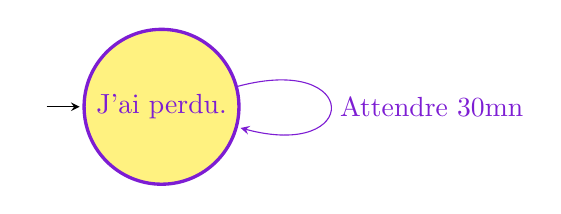
\begin{tikzpicture}[shorten >=1pt,node distance=1cm,>={stealth}, initial text = ,
        every state/.style={draw=vulm,very thick,fill=yulm!50, text = vulm}, accepting/.style={accepting by arrow, double}]
        \node[state, initial] (q) {J'ai perdu.};
        \path[->, vulm] (q) edge[loop right] node [right] {Attendre 30mn} (q);
    \end{tikzpicture}
    \caption{\textsc{Le Jeu}}
    \label{fig:dfa:lejeu}
\end{figure}


\begin{thebibliography}{5}
    \bibitem{game-rep-automata} A-Games: using game-like representation for representing finite automatas \textit{Cleyton Slaviero, Edward Hermann Haeusler}
    \bibitem{card-game-lang} A Card Game Description Language \textit{Jose M. Font, Tobias Mahlmann, Daniel Manrique, and Julian Togelius}
    \bibitem{cfgames} Active Context-Free Games \textit{Anca Muscholl, Thomas Schwentick, and Luc Segoufin}
    \bibitem{game-design-automata} Computing Game Design with Automata Theory \textit{Noman Sohaib Qureshi, Hassan Mushtaq, Muhammad Shehzad Aslam, Muhammad Ahsan, Mohsin Ali and Muhammad Aqib Atta}
    \bibitem{cfgames-sum} Summary for Context Free Games \textit{Lukáš Holík, Roland Meyer and Sebastian Muskalla}
    \bibitem{permut-grammar} Permutational Grammar for free word order languages, \textit{Mats Eeg-Olofsson and Bengt Sigurd}
    \bibitem{timed-automatas-games} Timed Automata for Video Games and Interaction, \textit{Jaime Arias, Raphael Marczak, Myriam Desainte-Catherine}
\end{thebibliography}


\end{document}

